%!TEX root = thesis_name.tex

% for wirting a thesis: use book and openright with twoside!
\documentclass[11pt, a4paper, twoside, openright, final]{book}

%%% input encoding
\usepackage{ucs}				% contains support for using UTF-8 as input encoding. Could in most cases be ommited
\usepackage[utf8x]{inputenc}	% use utf8 as document encoding.
								% Therefore, umlaute (ä,ö,ü,ß,...) could be used as they are, without any special latex commands

%%% language
\usepackage[german]{babel}	% english hyphonation and english as default language
								% change here to "ngerman" for automatic translation from "figure" to "Abbildung" and so on
\usepackage[german=guillemets]{csquotes} % German guillemets quotes

%%% better readable fonts
\usepackage{libertine}					% standard font
\usepackage[scaled=0.83]{beramono}		% monospace font
%\usepackage[libertine]{newtxmath}		% math font

%%% standard packages
\usepackage{float}				% float environments for images, tables, ... for flexible and better layouts
\usepackage{array}				% arrays, matrices, inner table environment
\usepackage[bf,small]{caption}	% captions beneath pictures; text smaller than normal text; "Figure" printed in bold
\usepackage{fancyhdr}			% add headers and footers to the document
\usepackage{ifthen}			% if-then-else constructions could be used; needed for redefining \cleardoublepage
\usepackage{multirow}			% span multiple cols, rows in tables
\usepackage{microtype}			% better typesetting
\usepackage{booktabs}			% nicer tables
\usepackage{enumitem}			% for correct indentations in long line items in itemize

%%% math
\usepackage{amsmath}			% better math output. needed for \dfrac = fracs in matrices
\usepackage{amsfonts}			% nice math fonts
\usepackage{amssymb}			% nice math symbols
\usepackage{amsthm}				% theorem definitions
\usepackage{units}				% units, i.e. \unit[23]{m} (23 meters)
\usepackage{nicefrac}			% smaller frac's due to diagonal line \nicefrac{1}{2}
\usepackage{mathtools}			% for shortinertext in equations with description

%%% graphics
\usepackage{graphicx}			% builds upon the graphics package (thus, is newer). offers more op­tional ar­gu­ments
\usepackage{grffile}			% graphic filename extensions
\usepackage{subcaption}		% multiple images in one figure environment. subfigure is deprecated!
\usepackage[usenames,dvipsnames]{color}		% some standard and predefined colors
\usepackage{tikz}				% draw stuff in LaTeX directly
\usepackage{colortbl}			% colour in tables

%%% links
\usepackage{url}				% clickable url's inside the text
\usepackage{hyperref}			% clickable inner-document hyperlinks (e.g. in Table Of Content) and e-mail-adresses

%%% computer science
\usepackage{listings}			% for printing sourcecode
\usepackage{algpseudocode}		% pseudo-code, \begin{algorithmic} environment
\usepackage{algorithm}			% float environment for pseudo-codes. i.e captions, labels, ...

%%% miscellaneous
\usepackage{todonotes}			% todonotes. very useful during the wirting process
\usepackage{hvfloat}			% tables in landscape format on portrait page (aka table turned by 90degree)
\usepackage{lscape}			% single page in landscape (Querformat)
\usepackage{pdflscape}			% lscape, if using PDFLaTeX
\usepackage{parskip}			% no indention on new paragraphs but new line - might not be good style for german texts...
\usepackage{alltt}				% like verbatime but interprets LaTeX commands
\usepackage{lipsum}			% filler text, e.g. \lipsum[3-8]
%\usepackage[left, displaymath]{lineno}		% line numbers; left,right,switch  ;  


%%% Thesis specific
\usepackage{changepage}			% change the margin of a single page, e.g. the title page to be horz. centered
\usepackage{titlesec}			% change style of headings
\usepackage[square, numbers]{natbib}		% references on literature, options: (round, square) and (authoryear, numbers)
%\usepackage[left=2cm,right=2cm,top=2cm,bottom=2cm]{geometry}	% change the page layout (Seitenränder)

%%% Line numbering
%\renewcommand\linenumberfont{\normalfont\tiny\sffamily\color{MidnightBlue}}	% default: \normalfont\tiny\sffamily		;		\normalfont\bfseries\small

%%% configure listing package; this is a complete list of all options of the listing package 
\definecolor{comment}{rgb}{0.12, 0.38, 0.18 }	% #3F6A4D	green
\definecolor{keyword}{rgb}{0.37, 0.08, 0.25}	% #5F1441	purple
\definecolor{string}{rgb}{0.06, 0.10, 0.98}		% #101AF9	blue
\definecolor{linenumbers}{rgb}{0.5, 0.5, 0.5}	% ???		gray
\lstset{
	language=Matlab,			% the language of the code
	%morekeywords={print, ...},	% if you want to add more keywords to the set
	%deletekeywords={...},		% if you want to delete keywords from the given language
	%escapeinside={\%*}{*)},	% if you want to add LaTeX within your code
	basicstyle=\tiny ,			% the size of the font that is used for the code
	backgroundcolor=\color{white},			% choose the background color	
	keywordstyle=\color{keyword}\bfseries,	% keyword style
	stringstyle=\color{string},				% string literal style
	commentstyle=\color{comment}\itshape,	% comment style
	numbers=left,				% where to put the line-numbers. (none, left, right)
	numberstyle=\tiny\color{linenumbers}, % the size of the fonts + style that are used for the line-numbers
	stepnumber=1,				% the step between two line-numbers. 
	numbersep=6pt,				% how far the line-numbers are from the code
	rulecolor=\color{black},	% if not set, the frame-color may be changed on line-breaks within not-black text (comments)
	showspaces=false, 			% show spaces adding particular underscores
	showstringspaces=false,		% underline spaces within strings only
	showtabs=false, 			% show tabs within strings adding particular underscores
	frame=single,				% adds a frame around the code
	tabsize=2,					% sets default tabsize to <x> spaces
	captionpos=b,				% sets the caption-position to bottom
	breaklines=true,			% sets automatic line breaking
	breakatwhitespace=true,		% if automatic break should only only happen at whitespace
	keepspaces=true				% keeps spaces in text, useful for keeping indentation of code (possibly needs columns=flexible)	
	%extendedchars=true,		% lets you use non-ASCII characters; for 8-bits encodings only, does not work with UTF-8
	%title=\lstname				% show the filename of files included with \lstinputlisting; also try caption instead of title
}




%%% graphic-path, itemize, chapter numbering, comments
\graphicspath{ {./pics/} }				% default path for pictures
\renewcommand{\labelitemi}{-}			% use a - instead of a circle in lists
\numberwithin{equation}{chapter}		% use chapter number within equations. Needs amsmath package
%\renewcommand{\theequation}{\thechapter--\arabic{equation}}	% use -- instead of . in equation numbering
\newcommand{\comment}[1]{}				% own command: write inline comments 


%%% tables; % change p{#1} to m{#1} for vertical centering or b{#1} for bottom
\setlength{\tabcolsep}{5pt}
\renewcommand{\arraystretch}{1.35}
\newcolumntype{L}[1]{>{\raggedright\let\newline\\\arraybackslash\hspace{0pt}}p{#1}}	
\newcolumntype{C}[1]{>{\centering\let\newline\\\arraybackslash\hspace{0pt}}p{#1}}
\newcolumntype{R}[1]{>{\raggedleft\let\newline\\\arraybackslash\hspace{0pt}}p{#1}}

%%% redefine \cleardoublepage to be without headings
\makeatletter
\renewcommand*{\cleardoublepage}{\clearpage\if@twoside \ifodd\c@page\else
\hbox{}%
\thispagestyle{empty}%
\newpage%
\if@twocolumn\hbox{}\newpage\fi\fi\fi}
\makeatother

%%% subsubsection numbering. default is 2 levels in both cases
\setcounter{secnumdepth}{3}  	% in text
\setcounter{tocdepth}{3} 		% in table of content

%%% math abbreviations. Symbols for real, natural and complex numbers. and identity matrix symbol
\newcommand{\R}{\mathbbm{R}}
\newcommand{\N}{\mathbbm{N}}
\newcommand{\C}{\mathbbm{C}}
\newcommand{\1}{\mathbbm{1}}

%%% Headings and Footer
\pagestyle{fancy}				% use custom headers and footers
\fancyhf{}						% clear all header and footer definitions so far
\lhead[\thepage]{\rightmark}	% header, left:		on even pages: page number  	| on odd pages: current section 
\chead{}						% header, center:	empty
\rhead[\leftmark]{\thepage}		% header, right:	on even pages: current chapter  | on odd pages: page number
\lfoot{}						% footer, left:		empty
\cfoot{}						% footer, center:	empty
\rfoot{}						% footer, right:	empty
\renewcommand{\headrulewidth}{0.4pt}	% line beneath heading
\renewcommand{\footrulewidth}{0.0pt}	% line above footer
\addtolength{\headsep}{0.3cm}	% add some extra space between the header and the text, because of the horizontal line
\setlength{\headheight}{13.6pt}	% otherwise errors on chapter pages


%%% information about the thesis -- is done manually for the title page
% but keep this for metainformation in the pdf
\author{Alexander Prull, alex.pr@gmx.de}
\title{Programmierung eines Browser-Plugins zur Anzeige von Datenschutzinformationen im PlayStore sowie Evaluation der PlugIn-Performance}
\date{\today} % This will not change the date on the title page!!!



\begin{document}
%\linenumbers	

%%% create an own title page that looks more nicely than the standard LaTeX one
\begin{titlepage}
	\begin{adjustwidth*}{}{-2cm}
		\begin{center}
			~\\		% ~\\ has to stand here to start a paragraph and to use spacing
			\textbf{\Huge \sffamily	Universität Leipzig	\\	\small ~					\\
					\large \sffamily	Fakultät für Mathematik und Informatik	 \\
										Institut für Informatik				\\}
			
			\vspace{0.3cm}
			\begin{figure}[H]
	        	\hspace{5.1cm}
	       		
\includegraphics[width=4cm]{siegel.png}
	        \end{figure}
	        \vspace{0.15cm}
			\textbf{\Large \sffamily -- Bachelorarbeit --}
			\vspace{0.5cm}
			
			 \textsc{ \LARGE
			Programmierung einer Browser-Extension zur Anzeige von Datenschutzinformationen im PlayStore sowie Evaluation der Extension-Performance}
			
			\vspace{1.0cm}
			\textbf{Author} \\
		Alexander Prull \\ 
		\href{mailto:ap62puny@studserv.uni-leipzig.de}{ap62puny@studserv.uni-leipzig.de} \\
		Institut für Informatik \\
		\end{center}
		
		\vfill
		
		\begin{tabular}{*{3}{C{4cm}}}
			\small \textbf{First Supervisor} & 
			\small \textbf{Second Supervisor} & 
			\small \textbf{External Supervisor} \\
			
			\small Prof. Nummer 1 & 
			\small Prof. Nummer 2 & 
			\small Extern Nummer 1 \\
			
			\small \href{mailto:ggg@informatik.uni-leipzig.de}{ggg@informatik.uni-leipzig.de} & 
			\small \href{mailto:ttt@uni-leipzig.de}{ttt@uni-leipzig.de} &
			\small \href{mailto:rrr.eee@uuu.com}{rrr.eee@uuu.com} \\
			
			\small Fancy Computer Science & 
			\small Institute of Rocket Science & 
			\small Something AG\\
		\end{tabular}
		
		\vspace{1.0cm}
		\centering{\today}
	\end{adjustwidth*}
\end{titlepage}
\cleardoublepage





\pagenumbering{roman}	% roman numbers: I, II, III, IV, V ... in front matter
\setcounter{page}{1}	% start with I in Abstract

\chapter*{Abstract}
\label{c:abstract}
In dieser Arbeit wird sich mit den Eigenheiten der Browser Extension Programmierung auseinander gesetzt. Speziell geht es um Extension die Webseiten um bestimmte Informationen erweitern. Diese werden von einem Backend empfangen und zur Ladezeit der Seite eingespeist. Dabei setzt sich die Arbeit mit zwei Punkten auseinander. In erster Linie geht es darum die Ladezeit der Webseite durch das Anfordern von Informationen so wenig wie möglich zu beeinflussen. Also die Performance der Extension zu maximieren. Auf der anderen Seite wird durch die Nutzung der Extension von einer steigenden Nutzerzahl der Backend-Server mit einer steigenden Anzahl von Anfragen belastet. Um diese Probleme zu lösen werden in der Arbeit verschiedene Möglichkeiten zur Speicherung von Daten betrachtet und eine Auswahl der Methoden auf ihre Performance hin getestet.

%%% end abstract
%%%%%%%%%%%%%%%%%%%%%%%%%%%%%%%%%%%%%%%%%%%%%%%%%%%%%%%%%%%%%%%%%



% show a table of contents (Inhaltsverzeichnis)
\tableofcontents
% add some blank pages
\cleardoublepage


\pagenumbering{arabic}	% arabic numbers: 1,2,3,4,5 ... when NOT in front matter
\setcounter{page}{1}	% start with 1 in first Chapter

%%% now add all sub-latex files here to form the complete document

% abstract is done directly in this file. see above
% add the single chapters from external files:
\chapter{Einleitung}
\label{c:einleitung}

Im Zeitalter der Digitalisierung werden große Mengen Informationen immer schneller und detaillierter verarbeitet. -?-  Jeder, der im Internet unterwegs ist, hinterlässt dabei wertvolle, persönliche Daten. Dabei spielt der Datenschutz eine wichtige Rolle, denn nicht immer werden diese Daten freiwillig preisgegeben. So reguliert die Datenschutzerklärung, welche Nutzerdaten verarbeitet werden. Denn in dieser Erklärung muss jeder Dienstanbieter dem "Nutzer zu Beginn des Nutzungsvorgangs über Art, Umfang und Zwecke der Erhebung und Verwendung personenbezogener Daten sowie über die Verarbeitung seiner Daten in Staaten außerhalb des Anwendungsbereichs [...] in allgemein verständlicher Form zu unterrichten"  (Telemediengesetz Paragraph 13 1 1)

Das Projekt Privacy Guard hat sich damit beschäftigt, inwiefern diese Datenschutzerklärungen den Vorgaben entsprechen und im Speziellen analysiert, welche Applikationen unvollständige oder mangelhafte DSEs vorweisen. Im Rahmen dieses Projektes entstand die Idee, bereits vor der Installation von Anwendungen, deren Datenschutzerklärungen zu untersuchen und den Nutzer auf mögliche Bedenken hinzuweisen.

\section{Aufgabenstellung}
\label{s:aufgabenstellung}

Die Arbeit befasst sich mit den folgenden Aufgaben:
\begin{enumerate}
	\item \textbf{''Programmierung einer Browser-Extension zur Anzeige von Datenschutzinformationen im PlayStore''}
	\item \textbf{''Evaluierung von Caching Methoden einer Browser Extension''}
\end{enumerate}

Hauptaugenmerk ist die Erläuterung von Browser-Extensions, Umsetzung eines Beispiels und Limitationen.
Welche Arten von Speicher stehen einer Extension zur Verfügung und welche Performance-Ersparnisse kann durch Abspeichern von Daten die die Extension wiederholt benötigt eingespart werden. Welche Entlastung erfährt der Server mit Backend. Aufbau und Einbindung des ausgewählten Kandidaten


\section{Aufbau der Arbeit}
\label{s:aufbauderarbeit}

Zu Beginn werden Recherche Ergebnisse vorgestellt und ausgewertet.  Aus den dadurch gewonnenen Resultaten die Aufgaben genauer Definiert. Auf Basis der Recherche entsteht im 1. Teil eine Extension wobei der Fokus darauf liegt, dass diese möglichst übersichtlich bleibt und zur Evaluierung von Speichermethoden dient. Anschließend werden verschiedene Testläufe präsentiert bei denen bestimmte Methoden zur lokalen Speicherung von Daten unter den gleichen Rahmenbedingungen verwendet werden. Die Ergebnisse werden verglichen und den Erwartungen gegenübergestellt. Zuletzt wird ein Fazit gezogen.


















\chapter{Vorarbeit}
\label{c:vorarbeit}


\section{Recherche zu Browser Extensions}
\label{s:recherchebrowserextensions}

\subsection{Extension-Programmierung allgemein}
\label{ss:extensionprogallg}

Unter einer Extension versteht man ein Programm, welches den Browser um neue Funktionen ergänzt. Durch eigene Oberflächen oder Manipulation der Website erleichtern diese Erweiterungen das Nutzen des Browser. 
Im Gegensatz zu Plug-Ins haben Extensions Zugriff auf Browser-spezielle Funktionen und sind in der Lage über die Webseite hinaus zu agieren. Plug-Ins werden direkt in eine Webseite eingebettet und sind auf diese beschränkt. Der Oberbegriff „Add-on“ wird heutzutage Hauptsächlich als Synonym für Extension verwendet.
Jeder größere Browser stellt eine Plattform zur Verfügung auf denen Extensions angeboten und installiert werden können. In der Regel sind Diese kostenlos. Können auch von außerhalb installiert werden zu Entwicklungszwecken oder wenn nicht auf der Plattform angeboten.
Extensions werden in HTML, JavaScript und CSS implementiert. Dabei können alle Bibliotheken verwendet werden, welche den Browserstandards für Extensions entsprechen. Kapitel 2.3.2 befasst sich genauer damit, welche Bedingungen für diese Bibliotheken in Google Chrome gelten.
Bekannte Beispiele sind Werbeblock wie UBlock Origin und VPN-Anwendungen wie Hola.

\subsection{Existieren bereits vergleichbare Extensions}
\label{ss:vergleichbareextensions}

Gesucht wurde nach einer Extension die auf der Play Store Seite den Nutzer datenschutzrelevante Informationen zu den angebotenen Apps liefert, Eine Datenschutzwertung im Playstore vergibt oder den Nutzer Apps nach Berechtigungen die Apps vorschlägt.
Extensions werden nach ihrer Kurzbeschreibung in den Suchergebnissen überprüft und bei nicht eindeutig Aufgabenbeschreibung die Infoseite aufgerufen(Bsp. Safe.ad im Web Store „ecosystem“).Nur deutsche und englische  Ergebnisse werden berücksichtigt.

Die Recherche hat ergeben, dass unter den genannten Suchkriterien keine Chrome oder Firefox Extension gefunden wurde die Aufgabenbereich der geplanten Extension abdeckt. Einige aufgeführte Beispiele implementieren einen Teil der geplanten Funktion (Umsortierung, Tracker checken) , aber keine Extension erfüllt alle gewünschten Aufgaben.


\subsection{Vergleich führender Browser als Plattform für die Extension}
\label{ss:vergleichbrowser}
Die getroffene Auswahl des Browsers als Plattform für die Entwicklung der Extension basiert hauptsächlich auf den aktuellen Marktanteilen. Google Chrome führt mit ca. 71\%, gefolgt von Mozilla Firefox mit 9,5\%, Microsoft Internet Explorer mit ca. 5,7\%, Apple Safari mit ca. 5\%, Microsoft Edge mit 4,4\% und Opera mit ca. 2,4\%.

\begin{figure}[ht]
	\centering
	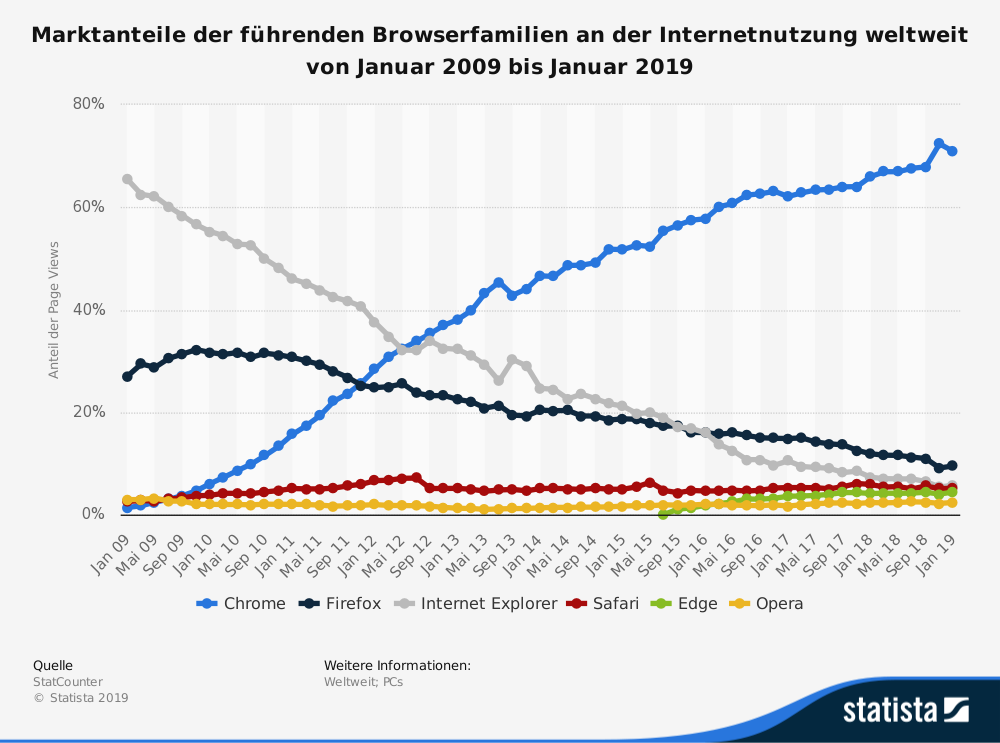
\includegraphics[width=1\textwidth]{pics/MarktanteileBrowser.png}
	\caption{StatCounter. n.d. Marktanteile der führenden Browserfamilien an der Internetnutzung weltweit von Januar 2009 bis Januar 2019. Statista. Zugriff am 4. März 2019. Verfügbar unter \url{https://de.statista.com/statistik/daten/studie/157944/umfrage/marktanteile-der-browser-bei-der-internetnutzung-weltweit-seit-2009/}.}
	\label{marktanteilebrowser}
\end{figure}
Aufgrund mangelnder Relevanz der Extension für Safari-Nutzer, sowie der Obsoleszenz des Internet Explorers, wurden diese Browser nicht weiter berücksichtigt.

Google Chrome ist den verbleibenden Alternativen Mozilla Firefox, Microsoft Edge und Opera im Punkt Marktanteile weit voraus und somit die gewählte Plattform zur Entwicklung der Extension.

Unabhängig der Implementierung bieten sowohl Mozilla\footnote{\url{https://developer.mozilla.org/en-US/docs/Mozilla/Add-ons/WebExtensions/Porting_a_Google_Chrome_extension}}, als auch Edge\footnote{\url{https://docs.microsoft.com/en-us/microsoft-edge/extensions/guides/porting-chrome-extensions}} eine intuitive Lösung zur Portierung der fertigen Google Chrome-Extension.

\section{PrivacyGuard}
\label{s:pguard}

\subsection{Vorstellung}
\label{ss:vorstellung}

\subsection{API-Anbindung für die Extension}
\label{ss:apianbindung}


\section{Implementierung einer Google Chrome Extension}
\label{s:implementierung}

\subsection{Eigenschaften}
\label{ss:eigenschaften}

Die Architektur einer Chrome Extension stellt ein Paket aus mehreren Dateien dar und ist vergleichbar mit anderen Web-Technologien wie zum Beispiel Webseiten.
Grundvoraussetzung für eine funktionierende Extension ist die manifest.json, welche grundlegende Informationen für den Browser bereitstellt und festlegt mit welchen Dateien und Rechten die Extension aufgebaut ist. Hinzu kommt mindestens eine HTML-Datei zur Darstellung der Inhalte und mindestens ein Skript zur Umsetzung der Funktionalität. Erweitert werden diese oft durch CSS-Dateien.
Externe Bibliotheken wie JQuery können ebenfalls eingebunden werden, müssen aber aufgrund der Policies von Google Chrome vollumfänglich lokal vorliegen. Mehr dazu Im nächsten Abschnitt.
Die Manifest-Datei ist im JSON-Format aufgebaut und beinhaltet sämtliche Informationen über die Extension. Wichtige Punkte sind Name der Extension, Beschreibung, Rechte und Aufbau. Unter Rechten oder „permissions“ werden alle APIs aufgelistet, welche die Extension benötigt um ordnungsgemäß zu funktionieren. Bevor ein Nutzer später die Extension installiert, muss er diesen „permissions“ zustimmen. Mehr zu den APIs im entsprechenden Abschnitt.
Der Aufbau wird unter „content scripts“ (BILD?) in drei Eigenschaften unterteilt: unter welchem URL sind die Skripte aktiv, welche Skripte sind dort aktiv und welche CSS-Dateien werden dort von der Extension eingesetzt.
HTML-Dateien werden als „User-Interface Elemente“ zusammengefasst und beinhalten im Normalfall eine popup.html zur Darstellung des Fensters der Extension in der oberen rechten Ecke des Browser-Fensters (BILD?). Je nach Funktionsumfang können weitere UI-Elemente eingebunden sein, um zum Beispiel die besuchte Webseite zu erweitern.

Die vorhandenen Skripte werden normalerweise in zwei Kategorien eingeteilt. Das sogenannte „Background-Skript“ dient als Event-Handler und kommuniziert zwischen Extension und Browser. Alle restlichen Skripte sind „Content-Skripte“. Sie beinhalten die eigentliche Funktionalität der Extension. 

\subsection{Funktionsumfang}
\label{ss:funktionsumfang}

\subsection{Darstellung im Browser}
\label{ss:darstellung}


\section{Caching-Methoden}
\label{s:cachingmethoden}

\subsection{Welche Rolle spielt Performance?}
\label{ss:rolleperformance}

\subsection{Verwendete Methoden und deren Eigenschaften}
\label{ss:methodeneigenschaften}




















\chapter{Hauptteil}
\label{c:hauptteil}

\section{Aufgabe 1: Implementierung einer Browser-Extension zur Anzeige von Datenschutzinformationen im PlayStore}
\label{s:implementierungextension}

\subsection{Anwendungsszenario}
\label{ss:anwendungsszenario}

%QUELLE STATISTIK? 

Während vor einigen Jahren Applikationen hauptsächlich auf eigenen Webseiten zum Download angeboten wurden, haben sich die
Appstores mittlerweile durchgesetzt. Vorteile für diese Plattformen sind unter anderem erleichterter Zugang, Vergleiche mit anderen Applikationen und individuelle Empfehlungen.

Bei der Wahl für eine bestimmte Applikation achten Nutzer auf Aspekte, wie Preis, Anzahl der Downloads und Bewertungen von anderen Nutzern. Immer wichtiger wird aber auch die Frage: Welche Daten gebe ich der Applikation frei und wie werden diese verarbeitet. Der PlayStore bietet zwar einen groben Überblick, welche Daten eine Applikation von dem Handy benutzt, aber nicht wie diese vom Anbieter weiterverarbeitet werden.

Außerdem sind Käufe von Apps in angelegten Benutzerkonten gespeichert. Mit diesem Benutzerkonto kann der Nutzer wiederum persönliche Daten für Login-Prozesse in Apps nutzen. So entsteht ein großes Netz an Informationen über das der Nutzer selbst keine Übersicht mehr hat.

Um Nutzern eine genaue Übersicht zum Datenschutz gewähren, betrachtet die Extension dabei Fragen,welche der PlayStore nicht unmittelbar beantwortet:
 \begin{enumerate}
 	\item \textbf{Handhabung der Daten}: Wie werden die Daten verarbeitet und an wen werden diese weitergeleitet? Wird ein Profil anhand der Daten erstellt? Welche Sicherheit besteht bei der Übertragung der Daten?
 	
 	\item \textbf{Vor- und Nachteile der Datenverarbeitung}: Kann der Anbieter die Applikation dadurch komfortabler gestalten? Wird Werbung in der Applikation personalisiert? Besteht Gefahr vor Missbrauch der Daten?
 	
 	\item \textbf{Kontrolle über die Daten}: Welche Möglichkeiten stehen zu Verfügung im Falle von Nichteinverständnis? Ist der Umgang mit den Daten nach der Installation noch einschränkbar. Kann der Nutzer die Verwendung der Daten verbieten und trotzdem die App weiterhin nutzen?
 \end{enumerate}

Ziel ist es Verbrauchern diese Fragen mittels der Erweiterung des Google PlayStores durch eine Extension zu beantworten.

\subsection{Anforderungsanalyse}
\label{ss:anforderungsanalyse}

\subsubsection{Funktionale Anforderungen}

Aus den Fragen, die bei dem Anwendungsszenario entstanden sind, werden funktionale Anforderungen gebildet um konkrete Aufgaben für die Extension zu schaffen. %-Anforderungen in TEXTFORM-

%-Direkt bei Apps in Anforderungen erwähnen
\begin{itemize}
	\item[/F10/] \textbf{Erweiterung der Informationen im PlayStore}:
	Der Nutzer hat die Möglichkeit im Browserfenster per Aktivierung bzw. Deaktivierung der Extension zusätzliche Datenschutzinformationen zu den angezeigten Applikationen ein- bzw. auszublenden.
	
	\item[/F20/] \textbf{Anzahl von bedenklichen Eigenschaften einer Applikation}:
	Zu jeder Applikation erhält der Nutzer ein Feedback von der Extension, wie viele Bedenken vorliegen.
	
	\item[/F30/] \textbf{Darstellung von kritischen Eigenschaften einer Applikation}:
	Eigenschaften einer Applikation, welche einen erheblichen Nachteil für den Nutzer darstellen oder einen möglichen Gesetzesverstoß beinhalten werden hervorgehoben.
	
	\item[/F40/] \textbf{Abrufen von Details zu den Bedenken}:
	Wird ein Bedenken angezeigt, kann der Nutzer direkt Erläuterung, Handlungsempfehlung sowie Vor- und Nachteile zu diesem Bedenken abrufen.
	
	\item[/F50/] \textbf{Empfehlung bei Suchanfragen}:
	Basierend auf den Bedenken einer Applikation kann der Nutzer die Suchanfrage so anpassen, dass ihm unbedenkliche Applikationen priorisiert angezeigt werden.
\end{itemize}

\subsubsection{Nichtfunktionale Anforderungen}

Das Programm richtet sich in erster Linie an Nutzer, denen keine besonderen informatischen Kenntnisse abverlangt werden.
Extensions zeichnen sich durch ihre Einfachheit aus. Nutzer wissen vor der Installation, welche Funktionen diese Programme haben. Die Extension soll auf den ersten Blick klar machen, welche Komponenten des Browsers erweitert oder verändert wurden.
%-QUELLE- Was ist eine Nichtfunktionale Anforderung + kurze Auflistung (BUCH)
\begin{itemize}
	\item[/NF10/] Darstellung und Einbindung der Informationen
	Darstellung und Einbindung spielen bei Browser-Extensions eine wichtige Rolle. Hier wird keine grundlegend neue Oberfläche gestaltet sondern eine bereits vorhandene erweitert. Der Fokus fällt darauf, die bestehende Oberfläche so zu verändern, dass alle Elemente der Extension an der richtigen Stelle eingebaut werden. Der Nutzer soll auf den ersten Blick erkennen welche neuen Informationen zu welchen bereits bestehenden Teilen der Website gehören.
	\item[/NF20/] Persistenz der Website
	Im Gegenspiel zu NF10 darf die Website nicht so verändert werden, dass sie in ihrem Aussehen und ihren Funktionen zu stark von ihrem Originalzustand abweicht. Gerade bei Seiten auf denen viele Elemente automatisch generiert werden, verursachen kleine optische Veränderungen schon Probleme beim Aufbau der Website. Entsprechend müssen Informationen so subtil wie möglich eingebettet werden. So wird verhindert, dass der Nutzer die Extension nur aufgrund der Optik wieder deinstalliert.
	\item[/NF30/] Handhabung
	In der Extension werden viele und vor allem auch umfangreiche Informationen angeboten. Diese dürfen den Nutzer nicht überwältigen. Dennoch müssen sämtliche Punkte vgl pguard informationen an der richtigen Stelle zur Verfügung stehen.
	\item[/NF40/] Skalierbarkeit
	def Skalierbarkeit? Hier bezieht sich der Begriff Skalierbarkeit vor allem auf Anfragen an das Backend. Angenommen die Extension erreicht eine hohe Nutzerzahl. Dadurch steigt das Risiko auf Überlastung des Servers. Um das zu verhindern werden bei der Informationsgewinnung zwei Aspekte besonders wichtig. Zum Ersten wie aktuell die Informationen sein sollen. Je aktueller, desto öfter müssen Anfragen gesendet werden. Zum Anderen die Relevanz. Wie schnell müssen welche Informationen vorhanden sein und welche Informationen, die eine Analyse erfordern, werden erst auf spezielle Anfrage des Nutzers angefragt. Diese Anforderung stellt einen zentralen Punkt in der Entwicklung der Extension dar und wird in Aufgabe 2 detailliert behandelt.
	\item[/NF50/] Datenschutz
	Bei allen Webdiensten spielt der Datenschutz eine wichtige Rolle. Auch in diesem Programm sollen Daten gespeichert werden um die Anforderung /NF40/ zu unterstützen. Um Datenschutzbedenken auszuschließen muss das Format der Daten so gewählt werden, dass diese nicht personalisert werden und nach Möglichkeit komplett lokal gespeichert werden.
	\item[/NF60/] Korrektheit der Daten
	Alle Informationen zu Applikationen die dieses Programm darstellt werden extern von einem Server des privacy guard-Projekts eingespeist. Dieser gewinnt die Daten hauptsächlich auf automatischen Textmining-Verfahren. Ein Problem bei diesen Verfahren ist die fehlenden Validierung der Informationen. Ursachen wie das heterogene Format von Datenschutzerklärungen und Mehrfachverlinkungen von Datenschutzinformationen können zu bei dieser Methode zu Fehlern oder Ungenauigkeiten führen. Aus diesem Grund muss dem Nutzer verdeutlicht werden, dass alle Angaben als Empfehlungen zu betrachten sind und keine verbindlichen Aussagen über Applikationen getätigt werden.
\end{itemize}
\subsection{Aufbau der Website}

Der Play Store, oder auch \glqq Google Play\grqq{} ist die Haupt-Vertriebsplattform von Google für digitale Güter wie Apps, Filme und Serien, Musik und Bücher. Diese Arbeit und somit die Entwicklung der Extension beschränkt sich auf die Kategorie Apps



%Singlepage, Multipage, Kacheln, APP-ID


Der in diesem Kapitel beschriebene Stand der Website bezieht sich auf den Zeitraum von März 2018 bis März 2019. Die Planung und Implementierung der Extension ist auf diesen optischen und technischen Stand der Website angepasst. Mögliche Probleme die ein veränderter Stand der Website mit sich bringt, werden in Abschnitt \ref{ss:diskussionht1} diskutiert.

\subsection{Programmaufbau}
\label{ss:programmaufbau}
Die Struktur des Programms orientiert sich an der beschriebenen Architektur in Kapitel~\ref{ss:darstellung}. Dieser Abschnitt befasst sich mit der Umsetzung der Anforderungen, welche im vorangegangen Kapitel aufgesetzt wurden. Dabei werden wichtige Eigenschaften aus an Teilen des Quellcodes betrachtet und getroffene Entscheidungen begründet. Außerdem werden kritische Stellen beleuchtet, welche für die Diskussion und fortführende Arbeit relevant sind.


\lstinputlisting[label={src:manifest}, caption={Aufbau der manifest.json}]{../../Extension/src/manifest.json}

Das Manifest stellt die grundlegenden Zusammenhänge der Extension dar. Unter anderem den gewählten Entwicklungsnamen der Extension "PGuard AppRating" und die entsprechende Beschreibung.
Weiterhin sind die nötigen Berechtigungen aufgeführt.
\begin{itemize}
	\item storage:
	Berechtigung zum Zugriff auf Speicherplatz, um Informationen aus Backend-Anfragen zu speichern. Details dazu in Kapitel~\ref{ss:anforderungen}.
	\item declarativeContent:
	Bereitstellung von Events, wie Seitenaufruf oder -änderung und damit zusammenhängende Regeln, wie das Ausführen von Content-Skripten. Diese API wird vom Background-Skript genutzt,welches die genannten Aufgaben umsetzt.
	\item activeTab und tab:
	Gibt an, ob sich der Nutzer gerade in einem Tab befinden auf dem die Extension aktiv ist.
\end{itemize}
Außerdem werden alle Dateien ihren Rollen zugewiesen.
\begin{itemize}
	\item Content-Skript:
	Unter dem Punkte "content scripts" wird festgelegt, welche Skripte unter welchem URL aktiv sind. Der Ausdruck 
	"*://play.google.com/store/apps*" 
	bedeutet, dass die Extension auf jeder Playstore-Seite der Kategorie Apps und deren Unterverzeichnis aktiv ist. Da es sich um eine page action Extension handelt, wird lediglich eine Website als "match" aufgeführt. Die beiden wichtigen Dateien hier sind "pguard.js" als das Content Skript für sämtliche Funktionen die die Erweiterung der Website betreffen und "popup-controller.js" für alle Funktionen des Popups. Hinzu kommen sämtliche Bibliotheken, welche von den Content-Skripten benötigt werden.
	\item Background-Skript
	Wie bereits erwähnt fungiert das Background-Skript "background.js" als Eventhandler der Extension ist deshalb separat im Manifest aufgeführt.
	\item web\_accessible\_resources
	Diese Ressourcen sind Dateien welche der Extension zur Verfügung stehen aber selber keine Skripte sind. Sie beinhalten ausgelagerte Informationen wie Fließtexte und Templates zum Bauen von HTML-Elementen. Die "popup.html" ist hier ein Sonderfall und wird direkt dem Popup zugewiesen.
\end{itemize}

Die Background.js besteht lediglich aus Callback-Funktionen der declarativeContent API. Hier wird zur Installation der Extension ein Listener eingebunden. Dieser funktioniert mit Regeln nach dem Konditionen-Aktionen-Prinzip. Zum Start des Aufrufs werden alle bereits vorhandenen Regeln des Listeners entfernt und anschließend die übergebenen Regeln installiert.
Hier benötigt das Programm eine Regel. Die Kondition prüft ob der passende URL aufgerufen wurde. Dieser stimmt mit dem String aus der Manifest-Datei überein. Ist die Kondition erfüllt, aktiviert sich das Popup.


\lstinputlisting[label={src:background}, caption={background.js}]{../../Extension/src/background.js}

Das Contentskript pguard.js bildet den Hauptteil der Extension und dient zur Erfassung aller, auf der Webseite dargestellten Apps, der Einbettung von zusätzlichen Informationen durch das PGuard-Backend und optischen Anpassung der Webseite, um die neuen Inhalte ordentlich einzubinden.

Bei Skript-Aufruf werden zuerst die lokalen Bibliotheken der Extension geladen. Dazu gehören die IB texte.json sowie die HTML-Templates. Außerdem überprüft das Skript, ob lokaler Speicher zur Verfügung steht. (???)

Anschließend prüft die Funktion "fillApps", ob die aktuelle Seite eine Single-App-Page oder Mutli-App-Page ist und ermittelt sämtliche Kandidaten, welche für die Einbettung der Informationen in Frage kommen. Dabei liest der JQuery-Selektor alle Elemente mit dem entsprechenden Klassnamen aus.

Mit der Funktion "loadInfoPanels" wird jeder so gefundene Kandidat auf seine APP-ID überprüft. Diese befindet sich entweder in dem Attribut "data-docid" oder "href". Mithilfe dieser ID durchsucht die Funktion "getStorageItem" den lokalen Speicher auf Einträge. Der  Eintrag ist valide, falls er nicht leer ist und vor weniger als 3 Tagen angelegt wurde. Findet die Funktion keinen validen Eintrag im lokalen Speicher, wird eine neue Anfrage an das Backend, für die entsprechende APP-ID, erstellt.

%BEISPIEL ANFRAGE

Liefert das Backend eine Antwort mit mindestens einem Ergebnis, speichert die Funktion die Informationen im lokalen Speicher ab. Bei mehr als einem Ergebnis, entscheidet eine Prioritätenliste abhängig von der zuverlässigsten Quelle, welcher Datensatz genutzt wird.

Der gewählte Datensatz wird der Funktion "createPanel" übergeben. Handelt es sich bei dem Kandidaten um eine App-Page(Single-App), wird das Popover aus den Informationen direkt erstellt. Dazu wird der Datensatz mit Hilfe der IB texte.json in den entsprechenden Text umgewandelt und in die Html-Template einfügt.
Bei App-Kacheln(Multi-app) baut die Funktion einen Banner in die Kachel ein. Auf diesem Banner wird mittels JQuery ein Event geladen, welches bei einem Klick auf den Banner das Popover erstellt.

%BEISPIEL IB texte
%\lstinputlisting[label={src:pguard}, caption={Aufbau der pguard.js}]{../../Extension/src/pguard.js}

\subsection{Ergebnis}
\label{ss:ergebnisseht1}

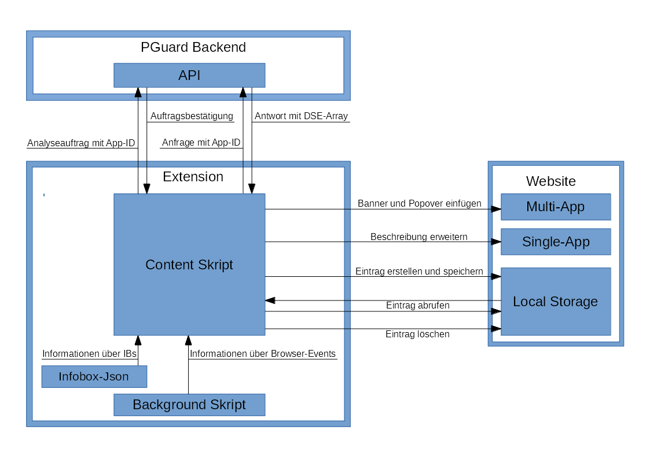
\includegraphics{pics/Aufbau.png}

\subsection{Diskussion}
\label{ss:diskussionht1}











\section{Aufgabe 2: Evaluierung von Caching Methoden einer Browser Extension}
\label{s:evaluierungcaching}


\subsection{Anforderungen}
\label{ss:anforderungen}
Extension erweitert die Landingpage.
Diese in Kategorien unterteilt. Kategorien werden bei jedem Besuch wieder aufgerufen
"Spiele mit Vorregistrierung" stellt über längere Zeit gleiche Apps dar.
"New + Updated Games" und "Top-Bewertung: Spiele" lieferen jedes Mal ähnliche Ergebnisse => überlappende Information
"Empfehlungen für dich" und "Das könnte dir Gefallen" passen sich vorherigen Suchen an und liefern daher auch redudante Ergebnisse
Selbe App oft mehrmals in der Übersicht vertreten
Konklusion: viel Redundanz. Ergänzende Information werden mehrfach benötigt

Verarbeitet Diese nur zu benutzerfreundlichen Format
Informationen müssen von externen Quelle entnommen werden
Dadurch entstehen Anfragen an einen Server mit Antworten
Antworten und Anfragen durch // redundant.

Thesen:
Nutzung der Extension nach "Veröffentlichung" würde hohen Traffic verursachen mit vielen wiederholten Anfragen.
Anfragen könnten ab einer bestimmten Nutzerzahl Server überlasten
Performance der Extension leidet unter dieser Art der Infortionsbeschaffung
Bei Ausfall der Quelle, bietet Extension keinen Mehrwert für den Nutzer mehr.

Lösung:
Einrichtung von unabhängigen Speicher zur Aufbewahrung der gewonnen Informationen. Insbesondere viele/wiederholt genutzt Informationen sollen ohne erneute Anfrage zur Verfügung stehen.
Neue Anfragen nur bei Veraltung der Informationen bzw. nur von neu aufgetauchten Apps
Aufbau einer Struktur zur Abspeicherung der wichtigen Informationen


Verwendung des Speichers:

Welche Informationen stehen pro App zur Verfügung?(1)
Welche Informationen werden pro App benötigt? (2)
Wie wird der Speicher gepflegt?(3)

(1)

Wird bei Aufbau der App schon Beschrieben?
Aynchron!

(2)
Alter der Information:
Ist die Information auf dem Aktuellen Stand wie die der Quelle?
Ist die Information der Quelle veraltet?
Wie oft wird so eine Information erneuert? (Neue DSE o.ä)
=> Abspeichern des Analysedatums. Regelmäßige Überprüfungen(3 Tage), ob neue Information bei der Quelle vorhanden

Aufruf der App:
Wie oft wird diese App aufgerufen?
Informationen über die App im Speicher können nach gewisser Zeit gelöscht werden, wenn sie nicht erneut aufgerufen wurde.
=> Frequency Count: Zähler im Speicher der bei jedem Aufruf erhöht wird. Regelmäßig wird der Speicher nach niedrigen Zählern durchsucht und diese Einträge gelöscht.

Informationen zur App:
Inhalt entspricht Kennnummern der Infoboxen. Also Abspeichern der jeweilig vorhandenen Eigenschaft/Infobox

(3)
LRU Konzept oder Fehler falls Speicher voll.
Aufbau des Speichers von Speichermethode abhängig (Chrome => key, value String)
Möglichst kurze Zusammenfassung der benötigten Informationen:
Alter der Information als Tageszähler seit festem Datum, da Tagesvergleich stattfindet
Frequency Counter als einzelner Integer (ÜB: casten auf einstellige Zahl "Protect"-Faktor?)
Abfolge von Kennnummer mit Infoboxen
Trennzeichen zum korrekten Auslesen der Informationen.
"ALTERTAGE(TRENNZEICHEN)FREQ(TRENNZEICHEN)IB(TRENNZEICHEN)IB ..."
Bsp: "17500|3|1|2|3|4"

FREQ FÄLLT WEG???

Worst Case:
99999|1|2|3|4|5|6|7|8|9|10|11|12|13|14|15|16|17|18|19|20|21|22|23|24|25|27|28|29|30|31
86 Character ~ 86Bytes

Limit = 5MB = 5242880 Bytes

5242880 / 86 = 60963 Einträge

Appanfragen pro Initialladen ~70


Nach Antwort von Server werden Informationen im Speicher abgelegt mit Startcounter.
Bei jedem erneuten Abrufen wird der Speicher abgefragt. Falls Information vorhanden und aktuell wird Counter angepasst und Informationen lokal ausgelesen. Ansonsten neue Anfrage an Server. Ist Antwort mit neuer Information vorhanden wird die alte gelöscht und durch die neue ersetzt.

Extension prüft in regelmäßigen Abständen den Counter-Status. Ist dieser zu niedrig wird die Information aus dem Speicher entfernt.

Speicher wird auf Maximalkapazität geprüft und eine Approximation vom "Füllstand" wird errechnet. Ist der Speicher voll, werden Einträge mit dem niedrigsten Counter gelöscht.



\subsection{Vorauswahl}
\label{vorauswahl}
Welche Arten von Speicher stehen einer Extension für Browser (hier Chrome) zur Verfügung?

Integriert: Session Storage und lokal Storage
Session Storage: Daten bleiben nur während der Sitzung erhalten. Das Schließen des Browsers bzw. das Öffnen der Website in einem anderen Tab/Browserfenster beendet die Sitzung

Local Storage: Daten bleiben über eine Sitzung hinaus erhalten und verfallen erst durch Überschreiben oder Löschen

Kapazität: 5MB

Aufbau: String-Tupel nach dem (Key, Value)-Prinzip

Zugriff: getItem(key), setItem(key,value) und removeItem(key)


Serverseitiger Speicher:
Identifizierung notwendig. Aufwendig in Pflege und Wartung. Kein Mehrwert zu Anfragen an Informationsquelle

Serverseitiger Speicher fällt vor vorne herein weg aus oben genannten Grund und datenschutzrechtlichen Bedenken.


Datenbanken:
Verfügbar: IndexedDB und WebSQL

WebSQL seit November 2010 von W3C nicht mehr empfohlen (veraltet).

IndexedDB: API in allen modernen Browser zur Speicherung von Daten und Dateien in einer object-orientierten Datenbank.
synchron und asynchron möglich.
Funktioniert nach key, value prinzip
Alle Datentypen von JavaScript werden unterstützt.
Kann indexiert werden um Suchen effizient zu machen.
Verwendet Prinzip von Transaktionen
Anfragen mit Rückgabewerten als Basis aller Operationen
Verfolgt den NoSQL-Ansatz


Speicherlimit nach global Limit (1/2 Festplatte) und Gruppenlimit (1/5 von global Limit, min 10MB max. 2GB)
Gruppenlimit voll = voll (Fehler)
Global Limit voll = löschen bis wieder frei (Quellenabhängig komplette Elemente gelöscht)

Warum nicht IndexedDB?

Vorteile von IndexedDB: Abspeicherung von großen strukturierten Datenmengen.
Nachteile: hoher Aufwand bei Implementierung.Overhead lohnt nicht bei kleinen Datenmengen. Transaktionen blockieren bei Fehlern  eventuell den Datenabruf bzw. die Aktualisierung

Storage API von Chrome ausreichend Speicher und geringer aufwand bei der Implementierung. Lediglich Strings benötigt. Indices bei gewählen value-Struktur nicht notwendig.

Vorteil von Session Storage: Speicherpflege nicht notwendig, da 5MB groß genug für Anzahl(?) an App-Informationen während einer Session im PlayStore. Informationen immer auf Stand der Quelle
Nachteil: Bei erstmaligen Öffnen des Stores in neuer Browsersession werden viele Anfragen losgeschickt für Apps die bereits in der letzten Session schon angefragt wurden. Bei Serverausfällen fehlen die Informationen
Lediglich in einer Session mehrfach aufgerufene Apps ersparen erneute Anfragen.
=> Speicherpflege fällt weg, dafür kaum Mehrwert bei Anfragen.

Vorteil von Lokal Storage: Apps werden einmal abgefragt und sind anschließend abgespeichert. Fällt der Server aus können die lokalen Informationen genutzt werden. Daten auch aus letzter Session bleiben vorhanden. Neue Anfragen werden nur dann geschickt wenn aktuelle Daten über 3 Tage alt sind.
Nachteile: Speicherpflege notwendig. Dadurch wird die Information länger (Counter und Tag). Zusätzliche Rechenzeit für das Löschen von alten Informationen notwendig. Dadurch wird sichergestellt dass die 5MB nicht überschritten werden und somit Informationen ungewollt verloren gehen. Für Informationen mit hohem Counter muss regelmäßig überprüft werden, ob die Information noch aktuell ist, weil diese in der Regel lange im Speicher verweilt.
=> Hohe Einsparung bei Anfragen an den Server möglich. Dafür müssen zusätzliche Operationen zur Speicherpflege und Prüfung der Informationen ausgeführt werden.

\subsection{Rahmenbedingungen}
\label{ss:rahmenbedingungen}

Plattform: Windows 10 Rechner Build, Specs
Chrome Details
App Details
Was wird gemessen?
Limitierungen

Getestet auf:

Windows 10 Education 64 Bit
Build 10.0.17134
Prozessor i7-6700K
RAM: 16GB
GPU: Nvidia GTX 1070

Chrome  67.0.3396.99 64 Bit


\subsection{Vorgehensweise}
\label{ss:vorgehensweise}



\subsection{Ergebnisse}
\label{ss:ergebnisseht2}

Storage: none
Ladezeit: 1435ms
Start der Extension-Funktionsaufrufe: 944ms
Dauer: 491ms
Anzahl der Anfragen an das Backend: 0


Storage: Local Storage
Ladezeit: 1711ms
Start der Extension-Funktionsaufrufe: 892ms
Dauer: 819ms
Anzahl der Anfragen an das Backend: 125


Storage: none
Ladezeit: 1761ms
Start der Extension-Funktionsaufrufe: 883ms
Dauer: 878ms
Anzahl der Anfragen an das Backend: 131




\subsection{Diskussion}
\label{ss:diskussionht2}
\chapter{Zusammenfassung der Arbeit}
\label{c:zsm}



\section{Zusammenfassung}
\label{s:zusammenfassung}

Im Rahmen dieser Arbeit entstand eine Browser-Extension zur Erweiterung des Google Play Stores um datenschutzrelevante Informationen. Dabei werden mit Hilfe des Backends von PrivacyGuard angezeigte Apps um Infoboxen mit Vor- und Nachteilen sowie Handlungsempfehlungen erweitert. Zusätzlich zeigen eingefügte Banner die Anzahl der Funde an und warnen den Nutzer vor sogenannten \glqq roten Linien\grqq{}.

Zu Beginn wurden dabei Recherchen angestellt, die zeigen, dass der Google Chrome Browser durch seinen hohen Marktanteil als Plattform am besten geeignet ist und keine Erweiterung mit den genannten Funktionen bereits existiert. Der zweite Teil der Vorarbeit hat sich mit dem genauen Aufbau und der Implementierung einer Chrome-Extension beschäftigt und welche Richtlinien dabei eingehalten werden müssen.

Anschließend wurde das Forschungsprojekt \textit{PrivacyGuard} vorgestellt zusammen mit dem Backend, welches als Quelle für Datenschutzinformationen dient. Um dieses Backend nicht zu überlasten, besteht der Bedarf eines lokalen Speichers in der Extension. Welche Methoden zur Verfügung stehen und sich für diesen Anwendungsfall eignen, wurde ebenfalls Teil der Recherche.

Aus den gewonnenen Informationen entstand eine Anforderungsanalyse mit funktionalen und nicht-funktionalen Nutzerszenarien für die Browser-Extension. Zur bestmöglichen Umsetzung wurde die Website des Google Play Stores betrachtet und eine möglichst einfache aber klare Darstellung der Informationen gewählt. Bis auf die Empfehlung bei Suchanfragen wurden alle Anforderungen umgesetzt und das Ergebnis anschließend betrachtet und einige Kritikpunkte diskutiert.

Nach der Implementierung wurden die recherchierten Caching-Methoden anhand bestimmter Kriterien verglichen und zwei Kandidaten für die weitere Evaluation ausgewählt. Diese Methoden wurde in die Erweiterung integriert. Messungen ergaben, dass die Extension durch das lokale Speichern von Informationen bis zu 67\% ihrer Ladezeit einsparen konnte, welche hauptsächlich durch Anfragen an das Backend beeinflusst wurde. Dabei lag die Caching-Methode \textit{indexedDB} vorne. Abschließend wurden Möglichkeiten diskutiert, um die Messungen zu erweitern und die Gesamtperformanz der Browser-Extrension weiter zu steigern.

\section{Ausblick}
\label{s:ausblick}

Während der Umsetzung der Aufgabenstellungen ergaben sich bereits Punkte, die aus zeitlichen oder organisatorischen Gründen nicht mehr umgesetzt werden konnten. Dieser Ausblick beschreibt eine mögliche Weiterentwicklung der Browser-Extension und neue Punkte zur Verbesserung der Performanz.

Der erste und wichtigste Punkt ist die Veröffentlichung der Extension. Um das zu ermöglichen bedarf es folgender Schritte:

\begin{itemize}
	\item \textbf{Wartung und Support}:
	Sowohl das Backend als auch die Extension müssen fortlaufend gewartet werden. Im Rahmen der Umsetzung der App kam es öfter zu Ausfällen im Backend aufgrund von Fehlern oder Speicherauslastungen. Auch die Extension selbst musste im Rahmen der Arbeit mehrmals angepasst werden, um alle Kacheln mit Apps zu erkennen. Auch neue Browser-Events wurden erst nach und nach entdeckt, was zu Lücken beim Laden von Apps führte. Nach einer Veröffentlichung benötigt die Extension also eine verantwortliche Person zur Wartung dieser und weiterer auftretender Probleme.
	\item \textbf{Evaluierung der Datenqualität}:
	Die automatische Datenverarbeitung läuft nicht durchweg zuverlässig und es treten hin und wieder Fehler bei der Ausgabe von Datenschutzerklärungen auf. Um nach der Veröffentlichung rechtliche Konsequenzen zu vermeiden und das Vertrauen der Nutzer nicht zu verlieren, muss die Qualität der Daten noch einmal überprüft werden.
	\item \textbf{Empfehlung bei Suchanfragen /F50/}:
	Stimmt die Datenqualität, kann auch das Nutzerszenario zur Empfehlung von alternativen Apps implementiert werden. Dadurch bekommt der Verbraucher Apps mit möglichst wenigen datenschutzrechtlichen Bedenken vorgeschlagen.
\end{itemize}

Optional kann die Extension auch auf andere Browser portiert werden. Dazu bieten Mozilla und Microsoft entsprechende Anleitung an(\cite{mozilla,edge}).

Gegen Ende der Bearbeitungszeit wurde eine weitere Methode zur lokalen Datenspeicherung veröffentlicht: \glqq File API \grqq{}\cite{file}.
Diese ermöglicht es Dateien anzulegen und als lokalen Speicher zu nutzen. Aktuell wird die API allerdings nicht vollständig von allen Browsern unterstützt. Eine weitere Evaluation könnte zeigen, ob das Vorteile in puncto Performanz gegenüber den in dieser Arbeit vorgestellten Caching-Methoden hat. 

Weiterhin wurde \textit{indexedDB} in dieser Arbeit ohne Frameworks umgesetzt. Unter Umständen bieten zum Beispiel \glqq localForage \grqq{}\cite{forage} oder \glqq Dexie.js \grqq{}\cite{dexie} eine bessere Performanz.

Abschließend sei erwähnt, dass mit der Veröffentlichung von Google Chrome Version 73 am 12. März eine neue Richtlinie eingeführt wird. Die sogenannte \glqq Cross-Origin-Resource-Policy \grqq{}\cite{corb} soll \glqq Spectre\grqq{}-Angriffe\cite{spectre} verhindern und vor kompromittierten Renderern schützt. Dazu können Http-Server über den Browser Anfragen von externen Seiten blockieren. Diese Richtlinie könnte auch Einfluss auf die Kommunikation zwischen der Extension und dem Backend haben und die API müsste entsprechend angepasst werden.














\chapter{Appendix}
\label{c:appendix}


\section{Derivations}
\label{s:appendic_derivations}



\newpage
\subsection{Example Matlab Code}
\label{ss:app_kalman_matlab}

Add a sourcefile directly into \LaTeX

\lstinputlisting[label={src:SimpleKalmanExample}, caption={Simple example of a Kalman Filter in Matlab}]{simple_kalman_example.m}













% acknowledgement is done directly is this file. see below
% bibliography is done directly is this file. see below



%%% Acknowledgement
\cleardoublepage
\chapter*{Acknowledgement}
\label{c:acknowledgement}

First of all, I would like to express my gratitude to ... for the aspiring guidance, useful comments and invaluably support throughout the whole process of this Master Thesis. Furthermore, I would like to thanks ..., ... and the other members of the research team for helpful discussions and constructive criticism. In addition, I would like to thank my University supervisor ... for all the helpful remarks, advises and discussions.

Also, I would like to thank my parents and ... who have supported me throughout the entire process by keeping me harmonious and motivated. 

Last but not least, I like to thank ... for funding my research and providing me with the facilities being required.



%%% list of all figures in this thesis
\listoffigures



%%% bibliography // references
\cleardoublepage
\bibliographystyle{abbrvnat}
\bibliography{papers}



%%% closing - conformation on non-cheating
\cleardoublepage
\chapter*{Proclamation}
Hereby I confirm that I wrote this thesis independently and that I have not made use of any other resources or means than those indicated.
\bigskip\bigskip\bigskip\bigskip\bigskip\bigskip\bigskip\bigskip
\begin{flushright}
	Forname Surname, Place, \today
\end{flushright}



\end{document}




































